\chapter{Methodology}
\label{methods}
%promises made in other sections:
% * description of disease enrichment method

%intro to the methods
This chapter describes the use of two probabilistic models to construct a weighted PPI network.
The first of these is a supervised binary classifier, implemented from a selection of either logistic regression, \ac{SVM} or random forest.
As the project progressed this method was unsuccessful and a second conditionally independent probabilistic model was used to update on prior knowledge and produce the final weightings.
Feature extraction was the predominant component in this project and involved turning the various data sources involved into usable features in a machine learning framework. 
%FIN: what would a non-traditional way be?  
The chosen Community Detection method, the fast and efficient Spectral Modularity algorithm, is also described. 
%FIN:why was it chosen? 

\section{Feature vectors}

%Features are the processed form of the data we use to make predictions about a given interaction between pairs of proteins and is defined mathematically in the following text.
The set of biologically relevant information associated with a given protein interaction is referred to as a feature vector and the constituent elements features.
The process of retrieving these from biological databases is referred to as feature extraction. 
%FIN: typo 
This is a task which commonly involved mapping between non-standardised protein identifiers and indexing large tables of biological data automatically.
%FIN: mention non-standardisation/alternative identifiers used in different data sources -I think you need to make it clear how difficult the data collection was especially as a novice to the available databases and data formats

% going through posing the problem in terms of probability
In supervised learning problems we wish to learn a mapping between input variables and output variables given a training set.
Defining this training set rigorously, it consists of input variables $\pmb{x}$, which are typically vectors of values known as features.
The output variables in a classification problems are a set of labels\autocite[2]{murphy_machine_2012} which are denoted as $y$.
In the case of binary classification these are simply either 0 or 1.
Given $N$ training vectors, $\pmb{x}_{i}$, corresponding to $N$ interactions in the network and training labels $y_{i}$ we can define our training set $\mathcal{D}$ for $N$ data points as:

\begin{align}
    \mathcal{D} = \left( ( \pmb{x}_{i}, y_{i} ) \right)_{i=1}^{N}
\end{align}

%an example?  

%pose our problem
Our problem involves taking various types of biological data, such as entries from biological databases indicating that proteins are involved in the same part of a cell and using these as features.
The training labels are either an interaction (a one) or a non-interaction (a zero).
Interactions are taken to be any interactions in the iRefIndex\autocite{razick_irefindex:_2008} consolidated database.
This database was chosen for reasons described in section \ref{gold}.
%FIN: why, what is this db? consolidated database
Non-interactions are random binary combinations of Entrez protein IDs, which is a method applied in other works\autocite{qi_evaluation_2006} to create negative training examples.
%FIN: created by you how and from what dataset, hell cite the script/ipynb you used
These are also checked against the iRefIndex database to ensure they are not accidentally known interactions.
The full training set contained 188,833 true interactions and 997,760 non-interactions, but only a sub-sample of this was used for training to ensure a ratio of 600 non-interactions per true interaction.
%There are approximately 600 non-interactions for every true interaction.

What we would like to estimate is the posterior probability of an interaction existing given a new feature vector after training our classifier.
%FIN: typo/missing word
For any model $\mathcal{H}$ and a new feature vector $\pmb{x}^{*}$ we can express this using Bayes theorem:

\begin{align}
    p(y^{*} = 1 | \pmb{x}^{*}, \mathcal{D}, \mathcal{H}) = \frac{ p(\pmb{x}^{*}| y^{*} = 1 , \mathcal{D}, \mathcal{H}) p( y^{*} = 1 | \mathcal{D}, \mathcal{H})}{ \sum{y^{*}} p( \pmb{x}^{*} | y^{*}, \mathcal{D}, \mathcal{H})}
    \label{eq:bayes}
\end{align}

Where in equation \ref{eq:bayes} posterior probability is $p(y^{*} = 1 | \pmb{x}^{*}, \mathcal{D}, \mathcal{H})$ and the prior is $p( y^{*} = 1 | \mathcal{D}, \mathcal{H})$.
Where $y^{*}$ and $\pmb{x}^{*}$ are a new label and feature vector, respectively.

We explicitly apply a prior to the probability of interaction based on the expected ratio of interactions to non-interactions stated in \autocite{qi_evaluation_2006}.
%FIN: what was Qi's justification for this value? Presumably observed ratios - cite the justifying paper if it wasn't Qi - unfortunately, it was Qi - other papers sometimes choose one in 350 or one in 400 (PIPs)
This is described in more detail in section \ref{bayes}.

\subsection{Protein identifier mapping}

Mapping from one protein identifier to another became a significant problem in this project.
%FIN: so a few of my earlier comments will be redundant to this section so reference from those sections to here 
Unfortunately, most Biological databases maintain their own indexing method to identify different genes and proteins.
New data sources being integrated into this project would often be using a different identification scheme to the NCBI Entrez GeneID originally chosen to use in the \ac{PPI} network.

%what the Entrez identifier is -  as opposed to other protein identifier schemes - cite NCBI web pages
Genes are defined by their amino acid sequence, but this is a long series of letters and the number of genes is much smaller than the possible combinations of these letters.
For the sake of posterity databases containing information about genes typically apply an identifier for each gene that is much shorter and can encode other information about the gene.
%FIN: commonly referred to as accessions 
The Entrez GeneID identifier is relatively simple, just consisting of a number generated when the gene was added to the database\autocite{maglott_entrez_2007}.

%other protein identifier schemes and mapping between them
Other popular schemes include the Ensembl identifier from the Ensembl database\autocite{hubbard_ensembl_2002}, Uniprot identifiers from the Uniprot database\autocite{consortium_universal_2008} and even those used only for specific databases such as \ac{DIP} identifiers\autocite{xenarios_dip_2002}.
Mapping between these different identifiers is difficult as each identifier may map to none or many in another database.
The reason this happens is due to isoforms of different proteins; different amino acid sequences can code for a protein with the same name.
%FIN: alternative splices of the same gene can produce different proteins, every gene is made of introns and exons, substrings which don't code for the amino acids in the protein and those that do respecitvely.  Expressed proteins are generated from any of several combinations of introns and exons (see http://en.wikipedia.org/wiki/Alternative_splicing).  Alt splicing is really important in eukaryotes and is one of the big explanations between the very low number of genes we found when we sequenced the human genome compared to the predicitions.
%FIN: the other source of 'isoforms' is when a piece of DNA is duplicated and have diverged a little in sequence between copies (older literature referred to alleles as isoforms which are slightly different as these are alternative forms of a gene such as say a gene for blue eyes or brown eyes (although that may actually be a polygenetic trait))
%FIN: you've also missed an issue with the multiple mappings of mistakes and errors, also these mistakes and errors being differentially fixed or propagated through databases.  A lot of the big source databases are public goods where many author's contribute and curation is mostly automated so have problems.  A fun and amusing example of finding accessions in databases that have been reformatted automatically by someone using excel and not noticing http://www.biomedcentral.com/1471-2105/5/80

%methods used during the project, with references to appendix notebooks
Various tools exist to map from one protein identifier to another: Ensembl's BioMart\autocite{smedley_biomart_2009} is a versatile web-based tool, for example.
In this project, simple conversion tables from NCBI's Gene\autocite{maglott_entrez_2007} ftp server were primarily used.
Another tool used was the Uniprot\autocite{consortium_universal_2008} online service web service.

% talk about the problem of canonicalisation
Unfortunately, using any of these services there will be a number of IDs which cannot be converted and many IDs mapping to the same Entrez ID as different protein isoforms are picked up.
%FIN: this isn't always the explanation - for example one database might contain say several different crystal structures done of a protein which will all theoretically map from many identifiers relating to each of these structures to one identifier of the raw sequence in genbank
One way to avoid this problem is to only refer to a single canonical form of any given protein and find this protein in other databases through its amino acid sequence.
%FIN: a benefit of this method is also that it can be used to find mis-labelled proteins: if you searched just for all data related to protein X, but someone had done a load of work on something they called protein Y but was actually protein X. If you didn't search by sequence you wouldn't find data 
This ensures that when referring to an interaction between two identifiers the interaction is always simply between two proteins.
%FIN: also note why the amino acid sequence is better than using the nucleotide sequence because it is the actual form of the protein and is derived after all the alternative splicing/isoform issues 

% how using Entrez identifiers risks becoming gene interaction prediction
% or "What Entrez isn't"
Otherwise, as in this project, the interaction is detected between two Entrez IDs; which corresponds to an interaction between genes - possibly only a single interaction between combinations of the isoforms of each gene.
%FIN: exactly, also worth putting the limitation in of not directly testing co-localisation and co-expression (i.e. temporal and spatial localisation allowing interaction)
Unfortunately, this means that this project is only concerned with gene interaction prediction until the Entrez IDs have been carefully canonicalized.
This is not really a problem, as we are only aiming to provide a weighting to a graph, rather than provide an accurate prediction of interaction between proteins.
%FIN: to be less negative maybe say you will still identify possible interactions but may not identify all of them (as you are only checking one isoform etc).  This can still be informative if it is a new predicition which is later validated

% how iRefIndex solves this problem and should have been used from the start
% with reference to storing the sequences of each protein involved to maintain unambiguity
A solution to this problem is provided by the iRefIndex\autocite{razick_irefindex:_2008} database, which combines many databases and stores canonicalized entries.
Using this database, it would be possible to ensure that the proteins used in a future project would be reliable canonical proteins.
Additionally, each protein of interest should ideally be stored with reference to its sequence in, for example, FASTA format.
%FIN: be explicit amino acid sequence rather than protein sequence

%description of feature extraction code
\subsection{Dedicated code: ocbio.extract}

% link to the notebook on using this code
% but update it to explain what custom generator options are
To keep track of the various different data sources and assemble the features into vectors to be used in the classifiers a dedicated piece of code was required.
The code developed is written as a python module called ocbio.extract.
Usage and development notes for this program are referenced in Appendix \ref{app:ocbio}.

\subsection{Gold standard datasets}
\label{gold}
%material on the problems with choosing between gold-standard datasets
% with reference here to the section in Qi's thesis


%original work on \ac{DIP} (justified choice from previous work)
The database of interacting proteins (\ac{DIP}) is a database of interactions proven by small-scale experiments\autocite{xenarios_dip_2002}.
Each interaction added is hand curated so it was expected as a reliable training set.
Also, this database was used as a training set in \textcite{qi_evaluation_2006}.

%problems with \ac{DIP}
%why \ac{HIPPIE} is better suited
Unfortunately, problems were found with \ac{DIP} as a training set. 
%FIN: I don't understand - explain what these problems are/were
Features derived from interaction databases would win out in importance versus all indirect features as shown in figure \ref{fig:unbalanced}.
\ac{HIPPIE} was also tested as a training set, but this lead to the same problem.
%FIN: so which did you use?

%example feature importance graph
\begin{figure}
    \centering
    \setlength\figureheight{3in}
    \setlength\figurewidth{4in}
    \InputIfFileExists{\imagedir/unbalanced.weighting.tikz}{}{\textbf{!! Missing graphics !!}}
    \caption{An example of an unbalanced set of feature importances plotted after fitting a Random Forest classifier to a dataset containing interaction database derived features. Feature indexes are not as described in table \ref{tab:fvectors}.}
    \label{fig:unbalanced}
\end{figure}

%After removing interaction databases 
It was decided that only indirect features should be used in the trained supervised classifier and direct evidence integrated into the final weightings in an explicit Bayesian method described in section \ref{bayes}; the results of which are described in section \ref{bayesresults}.
Once these databases were removed the performance of the classifier was drastically lower.
However, all of the available features had more closely distributed importances in the final classifier, as shown in section \ref{importances}.
%FIN: this isn't obvious to me - you need to explain why balance set of features is important 


%iRefIndex as a final solution?
To train the final classifier the iRefIndex\autocite{razick_irefindex:_2008} database was used to find positive interactions due to its effective protein identifier mapping ability, as described above.
Again, non-interactions were generated as random combinations of Entrez Gene IDs.
These were also checked against the positive interactions to ensure known interactions were not present.

\subsection{\ac{PPI} prediction features}

%planned features, describe the list of possible features which was created
%put it in the appendix as a table, or otherwise somehow
\ac{PPI} prediction features are a set of values for each interaction considered, if it is a real or non-interaction.
This arrangement is illustrated in figure \ref{fig:fvectors}.
The features used are described by index in table \ref{tab:fvectors}.

%this could be a good place to put that diagram of exactly what a feature vector is
\begin{figure}
    \centering
    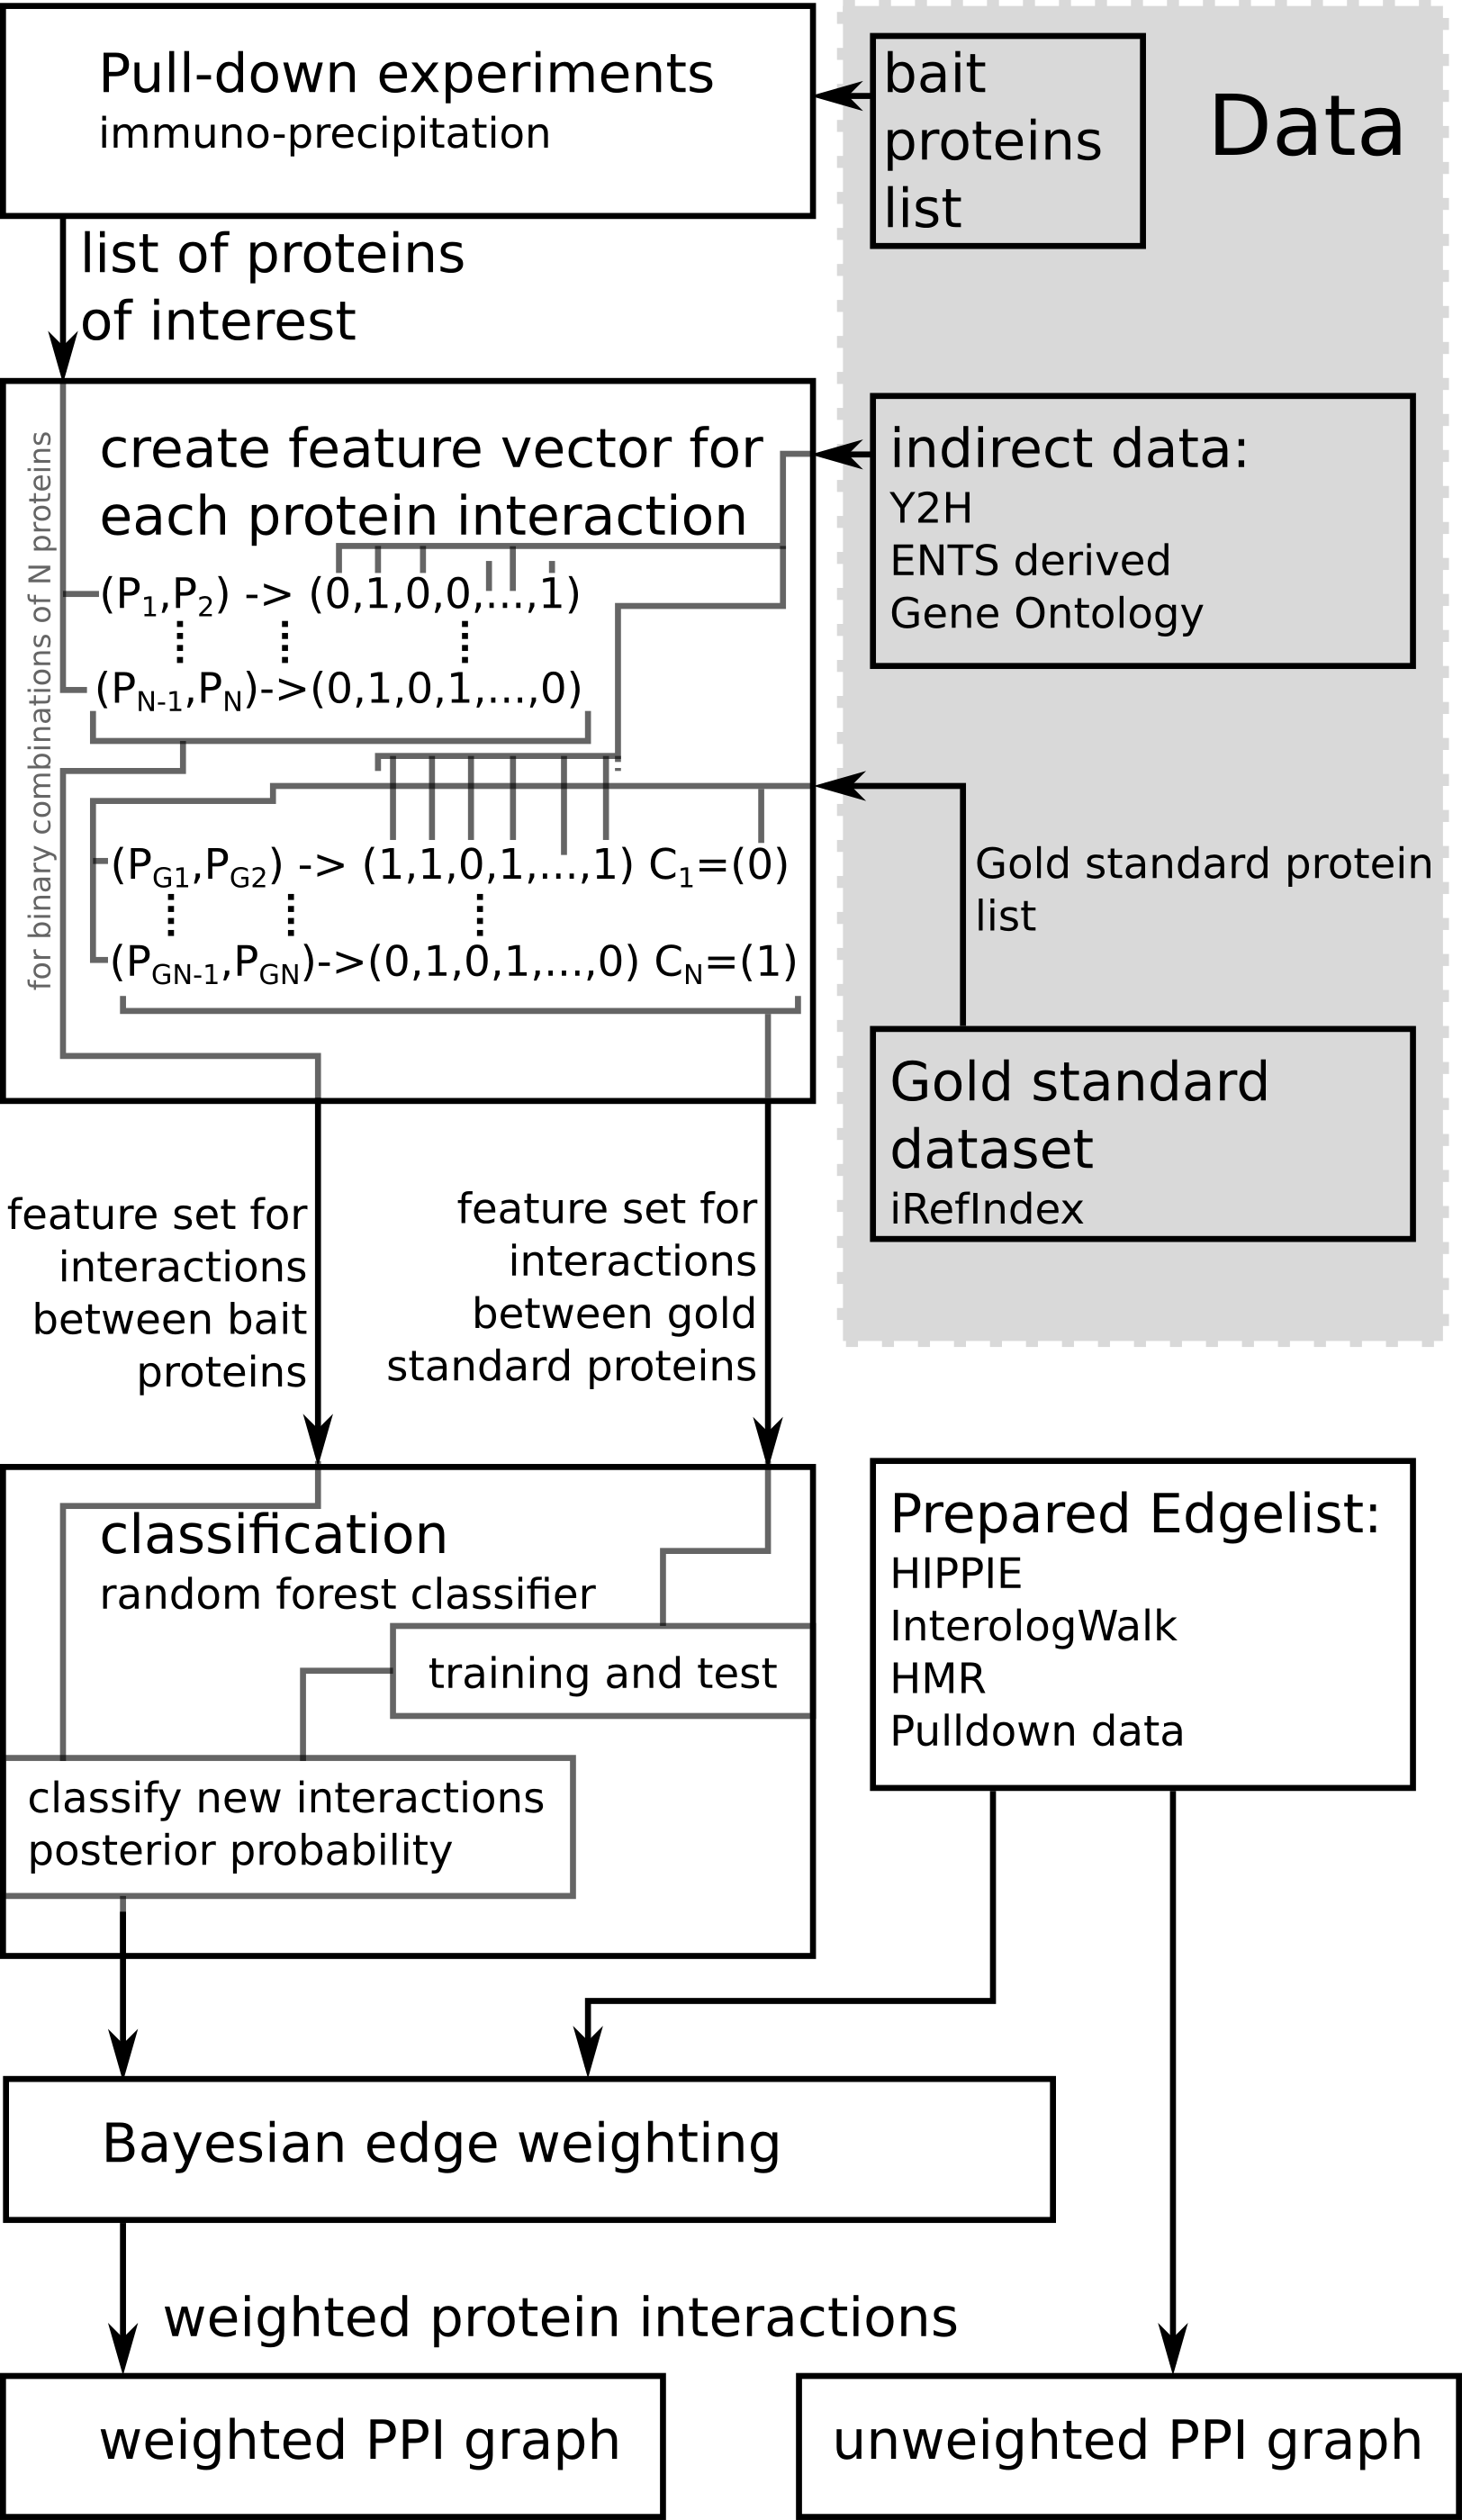
\includegraphics[width=0.8\textwidth]{fvectors.png}
    \caption{A diagram showing the structure of feature vectors and their relationship to the project as a whole. This figure is based on a similar flow chart shown in the project proposal.}
    \label{fig:fvectors}
\end{figure}

\begin{table}
    \centering
    \begin{tabular}{l c p{0.5\textwidth}}
        Feature         & Indices & Description \\
        \hline
        Gene Ontology   & 1-90    & Described in section \ref{go}, with individual indices described in Appendix \ref{app:go}. \\
        Y2H             & 91      & Y2H experimentally derived feature \\
        ENTS derived    & 92-198  & Features used by the ENTS classifier, described by index in supplementary table for \textcite{rodgers-melnick_predicting_2013}. \\
        ENTS summary    & 199     & Prediction result of the classifier in \textcite{rodgers-melnick_predicting_2013}. \\
    \end{tabular}
    \caption{Each feature used in the final classifier is described by index.}
    \label{tab:fvectors}
\end{table}

%details of what classifiers were chosen and about scikit-learning
\section{Weighting Protein Interactions}

%classification as a weighting tool
The classification problem we are solving is different in that we are really trying to obtain a realistic weighting of interactions for use in a \ac{PPI} network.
%FIN: different from what? 
Classification is normally concerned about picking a decision threshold to classify examples into categories.
However, in this case the output of our process is the posterior probability of the model given a new example.

%introduce scikit-learn
To produce this output the chosen tool was the Python package Scikit-learn\autocite{pedregosa_scikit-learn:_2011}.
Each classifier implemented in this package has a similar interface allowing modular code to be written.
In addition, this package is actively developed with all the required classifiers having efficient implementations.
%FIN: also one of most widely used packages 
% explain why we tried the algorithms that we tried
The following sections describe the three classifiers chosen.
These were a logistic regression model, a random forest model and a support vector machine.
Each of these involved tuning a number of hyper-parameters.

\subsubsection*{Hyper-parameters}
%describe the different parameters varied in scikit-learn by name
%FIN: explain what a hyper-parameter actually is  
Each of the Classifiers used has hyper-parameters which will affect its performance.
These hyper-parameters are described in table \ref{tab:hyper} for each of the models used in the project.
The optimal values for these found can be found in section \ref{gridresults}, table \ref{tab:gridresults}.

%table of the different hyper-parameters
\begin{table}
    \centering
    \small
    \begin{tabular}{p{0.2\textwidth} c p{0.5\textwidth}}
        
        Classifier                                  & Hyper-parameters     & Description \\
        \hline
        Logistic Regression                         & C                         &  Inverse of regularisation strength, the $\alpha$ parameter in section \ref{logreg}. \\
        \hline 
        \multirow{3}{*}{\parbox{0.2\textwidth}{Support Vector Machine}}     & kernel                    &  The kernel used. Three options: linear, \ac{RBF} and polynomial. \\
                                                    & Gamma($\gamma$)           &  Kernel coefficient. \\
                                                    & C                         &  As with Logistic Regression, a penalty parameter. \\
        \hline 
        \multirow{2}{*}{\parbox{0.2\textwidth}{Random Forest}}              & N estimators              &  Number of trees used in the forest. \\
                                                    & Max features              &  Number of features considered when looking for splits, part of the problem of finding the best decision at each node described in section \ref{randomforest}. \\
        \hline 
        \multirow{2}{*}{\parbox{0.2\textwidth}{Extremely Randomized Trees}} & N estimators              &  As with Random Forest. \\
                                                    & Max features              &  As with Random Forest. \\
    \end{tabular}
    \caption{Summary of the hyper-parameters described in the Scikit-learn \autocite{pedregosa_scikit-learn:_2011} documentation to be tuned for each of the models considered.}
    \label{tab:hyper}
\end{table}


\subsubsection*{Logistic Regression}
\label{logreg}

%with reference to Murphy
Logistic regression is a linear model being used for classification.
%FIN:binary classification  
It is equivalent to a linear regression model transformed through a sigmoid function\autocite[376]{murphy_machine_2012}, denoted here by $\sigma$:

\begin{align}
    p(c=1|\pmb{x}) = \sigma(b + \pmb{x}^{T}*\pmb{w})
    \label{sigmoidtransform}
\end{align}

In equation \ref{sigmoidtransform} $\pmb{x}$ is the vector of features and $c$ is the class label - in our case $1$ is a real interaction, $0$ is a non-interaction.
The weights and biases are the parameters of this model, expressed in the above equation as $b$ and $\pmb{w}$, respectively.

This divides the points in the dataset by a hyperplane, classifying the points on each side into different classes.
For data that is linearly separable, this produces a classifier that will make no mistakes on the test data.
Unfortunately, the data we are working with is not linearly separable as shown in section \ref{dataviz}.

%How is it trained?
To find the parameters the log likelihood of this model must be maximised; corresponding to the maximum likelihood solution.
The log likelihood for this model, for N feature vectors, is:

\begin{align}
    L(\pmb{w},b) = \sum_{n=1}^{N} c^{n} \log \sigma(b + \pmb{w}^{T}\pmb{x}^{n}) + (1 - c^{n})\log (1 - \sigma(b + \pmb{w}^{T}\pmb{x}^{n}))
\end{align}

%describe what the C parameter is
Regularisation of the weights represents a prior belief that the weights should not increase without bound.
In a case where the data is linearly separable and where regularisation is not applied the weights will increase without bound to produce extremely confident classifications\autocite[381]{barber_bayesian_2013}.
To stop this from happening we apply a penalty term, $\alpha$, to the size of the weights:

\begin{align}
    L'(\pmb{w},b) = L(\pmb{w},b) - \alpha \pmb{w}^{T}\pmb{w}
\end{align}

Tuning this hyper-parameter is the goal of a grid search when training a Logistic Regression model.
%FIN: explain grid-search 
\subsubsection*{Support Vector Machines}
%FIN: you are a big fan of Murphy 
%with reference to Murphy
Logistic regression can be generalised to apply kernel functions to the input features to obtain better classifications.
Support Vector Machines exploit this while also applying a different objective function intended to avoid overfitting\autocite[383]{murphy_machine_2012}.
The objective in placing the hyperplane for a Support Vector Machine is a "maximum margin" in that is attempts to maintain the same distance from the closest opposing class points.
%FIN: typo/missing word

%success of these models?
These are often successful classifiers in practice.
Applications include text categorisation, hand-written character recognition, image classification and biosequences analysis\autocite{cristianini_introduction_2000}.

%describe the hyper-parameters?
The hyper-parameters for a Support Vector Machine control the kernels, along with the regularisation parameter as described for logistic regression in section \ref{logreg}.
%FIN: explain what a kernel is and how \ac{SVM}s can classify non-linearly seperable unlink logit by transformation to feature space
Two hyper-parameters which can be tuned during a grid search operation are the degree of polynomial kernels if chosen and the gamma coefficient of the kernels.


\subsubsection*{Random Forest}
\label{randomforest}

Random forests operate as a combination of many decision trees.
Decision trees are intuitively simple in that it consists of a series of comparisons arranged in a tree as shown in figure \ref{fig:dectree}.

\begin{figure}
    \centering
    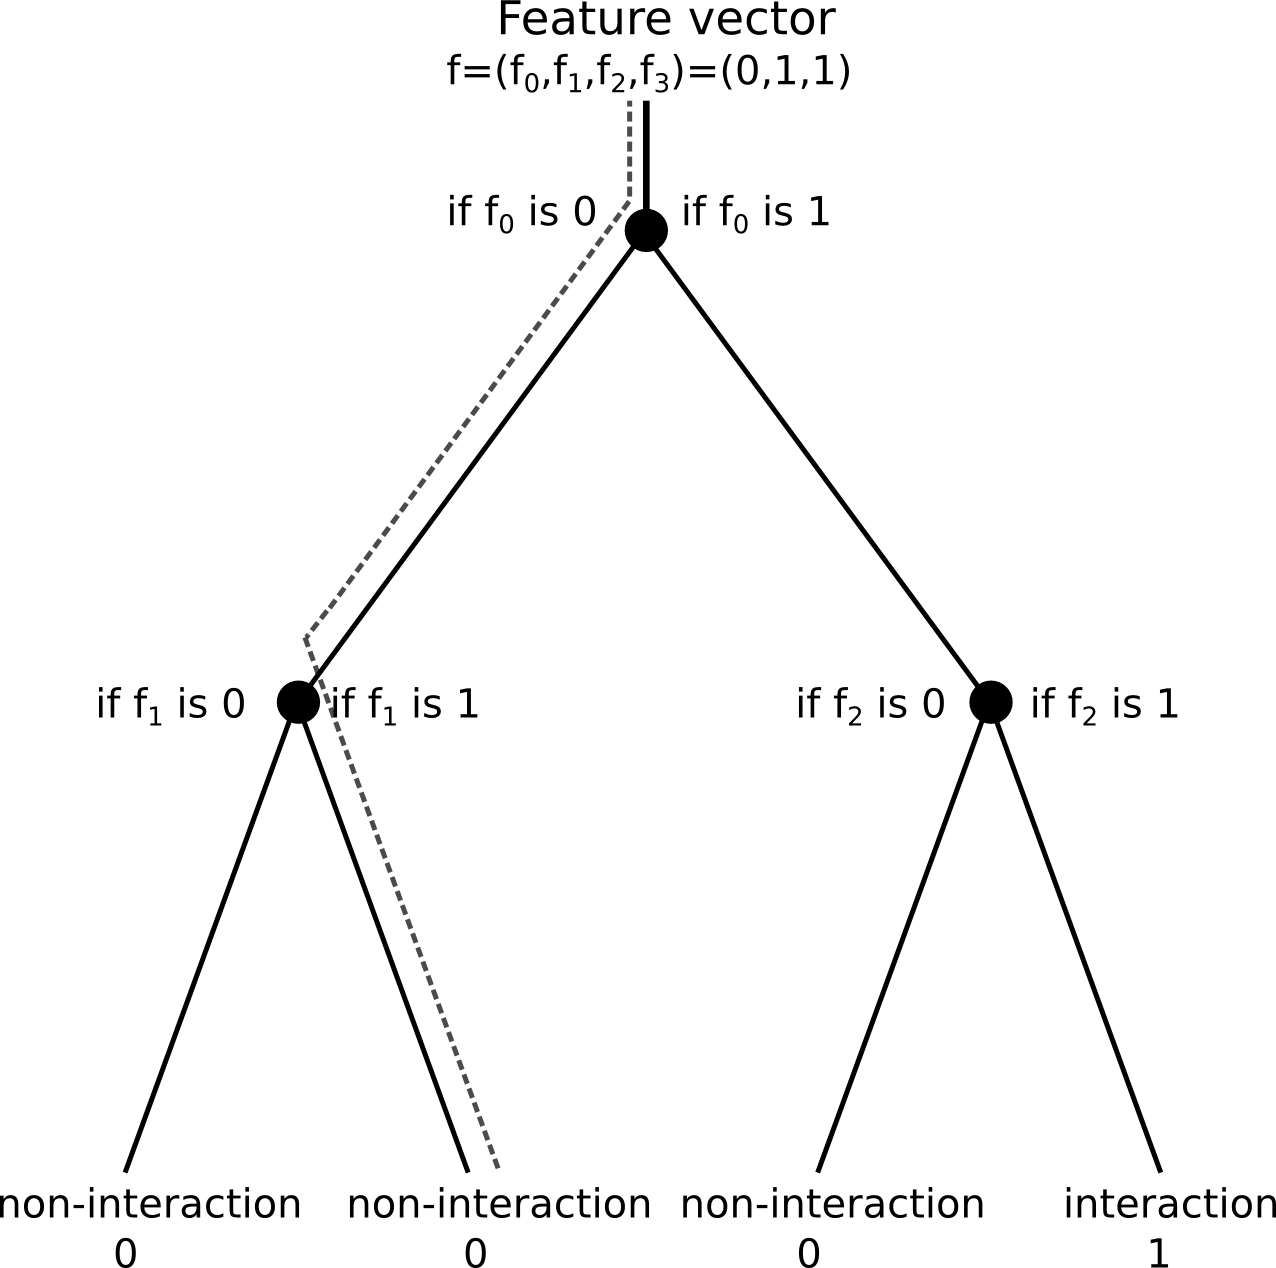
\includegraphics[width=0.8\textwidth]{decisiontree.png}
    \caption{A simple example decision tree, illustrating the process of sequential, dependent decisions. Based on an image obtained through Wikimedia\autocite{wkmdacommons}.}
    \label{fig:dectree}
\end{figure}

In this way decision trees are both simple and tractable methods for using a feature vector to classify inputs and there are many automated ways to generate effective decision trees.
The problem in the design of a decision tree is which comparison to choose at each node, described as how to partition the data\autocite[544]{murphy_machine_2012}. %redundant citation here?
There are several implementations of algorithms to achieve this and a full description can be found in \textcite[544]{murphy_machine_2012}.
Other advantages of decision trees include the ability to handle a mixture of discrete and continuous inputs, automatic variable selection, scaling to large datasets readily and the ability to handle missing inputs, with modification.
%other strengths of decision trees?

%describe split function? probably not worth going into this.

%then explain the problems with decision trees, variance etc
Unfortunately, despite the strengths of decision trees there are still problems with stability: small changes in the input data can produce large changes in the output\autocite[550]{murphy_machine_2012}.
The random forest algorithm addresses this problem by providing redundancy; multiple trees are grown and their results averaged.
%FIN: how many trees?
For M trees trained on different subsets of the data\autocite[551]{murphy_machine_2012}:

\begin{align}
    f(x) = \sum_{m=1}^{M} \frac{1}{M} f_{m}(x)
\end{align}

Where $f_{m}(x)$ is $m$th tree. This is simply averaging the results of the trees and is known as bagging.

%with reference to Qi and ENTS, showing good performance on this problem
With the ability to work on large datasets and mixing continuous and discrete data these types of classifiers would appear to already be well suited to this problem.
%FIN: maybe say well theoretically suited and then show in reality with the citations 
This is what has been observed in the literature, with these classifiers achieving the best performance despite different types of biological data being used\autocites{qi_evaluation_2006,rodgers-melnick_predicting_2013}.
Due to these reports in the literature it appeared that this classifier would be the best choice for our protein interaction prediction task.

%expand on how much better they were etc? in different places?

\subsubsection*{Other options}

% what other algorithms could we have tried but didn't
Other options considered for our classification problem, but not included in the project due to time constraints included Feedforward neural networks, Naive Bayes and Beta regression.
Naive Bayes in particular would have required modifying the code from Scikit-learn to deal with data from multiple different distributions or implementing Weka's solution of kernel density estimated distributions for each different feature\autocite{john_estimating_1995}.
%FIN: explain why 
Beta regression would have been very suitable for the task and is suggested as future work, described in the following section.

\subsubsection*{Beta regression}

%what is beta regression? quickly
Beta regression is a generalised linear model is one in which the output variable is distributed according to a Beta distribution\autocite{smithson_better_2006}.
%FIN: typo/missing word
A maximum-likelihood solution to this model can be found and the resulting model fit in the same way as a standard regression model.
%FIN: typo/missing word

%why this would also have been a good idea, if we didn't have to implement it ourselves
True protein interactions are not something which can be assumed in a protein interaction prediction task.
Many proteins are known to be very likely, but others are less confidently classified, as reflected in the \ac{HIPPIE} database's confidence scoring system\autocite{schaefer_hippie:_2012}.
%FIN: typo/missing word

To train a classifier a training set of true and false interactions is required and this cannot be supplied without thresholding the database at an arbitrary confidence value.

Beta regression avoids this problem as it allows the confidence values to remain a part of the regression process.
Using this we can build a model and update our belief on the likelihood of interaction in a Bayesian framework much more easily.

%FIN: actually this is pretty cool, note to self read up on Beta regression 
\subsection{Classifier testing}
\label{classifierverification}

%Tests we planned to use on each classifier:
%  mention cross-validation
%  learning curves
%  simple accuracy value
%  grid search
%  \ac{ROC}
%  Precision recall
%  test interactions
%  

% consider using paragraph headings in this section
Various measures were applied to each classifier to estimate their performance in different ways.
These tests included simple accuracy measures applied over learning curve and grid searches along with plotting \ac{ROC} and precision-recall curves.
Grid searches of parameter values were used to find optimal hyper-parameters.

% was or will be?
Cross-validation was applied to tests during parameters searches and when plotting learning curves to get a statistical estimate of the reliability of the metrics applied to the classifier\autocite[152]{witten_data_2011}.
%FIN: you don't really explain what CV and why you can't just optimise the models performance directly on the test set
As the training set is relatively large, these were applied as random sub-samples of the full data set, but stratified to maintain the same proportion of zeros to ones as in the full training set.
This is important as it must reflect the expected ratio for real protein interactions to non-interactions.

\subsubsection*{Pipeline}

%what is a pipeline? why did I use one?
A pipeline is a combination of algorithms intended to run on the data in sequence after the data has been split into training and test.
In the case of this project the pipeline involved three components: a mean value filling imputer, a standard scaler and the classifier itself.
The imputer simply replaced missing values in the training data with the corresponding mean value for that column.
Scikit-learn's standard scaler centers the data at zero mean and unit variance.

%FIN: need to explain/just why you need to normalise data and gracefully handle missing data

\subsubsection*{Learning Curves}
% learning curves, what are they? and why?
Learning curves, as in the notebook referenced in Appendix \ref{app:classtrain}, were used in this project to ensure that the number of samples used in a grid search was sufficient.
The learning curve plots the accuracy of a classifier after it has been trained using cross-validation on a varying number of samples.
%FIN: most importantly they can diagnose common classifier issues (bias/variance) 
%example learning curve?
%still pending, worth it if page count allows

\subsubsection*{Grid search}
% grid search
A grid search is a cross-validated test measuring accuracy testing the classifier with a variety of different hyper-parameters.
Classifiers, such as a Logistic Regression model, have some number of hyper-parameters.
A Logistic Regression model, for example, has a single hyper-parameter so that the grid search for this model simply involves varying this parameter to obtain the optimum performance on the test set.
%FIN:repeat hyper-parameter identity in logististc regression - regularisation

\subsubsection*{Accuracy}
% accuracy value
The accuracy value plotted in the learning curve and used in grid searches of parameters values is simply the proportional of correctly classified instances in a training or validation set.
Typically, the protein interaction prediction problem is sparse, in that there are very few interactions for the large number of non-interactions.
This is reflected in the accuracy in that a classifier that simply always predicts zero can still achieve a very high accuracy.
Using this accuracy value is therefore problematic and this requires the other measures employed, such as \ac{ROC} and precision-recall \ac{AUC} values.

\subsubsection*{\ac{ROC} curve}
% explain what those are
A Receiver Operating Characteristic, or \ac{ROC}, curve plots the variation in true positive to false positive rate as the threshold of classification is varied.
This makes it useful as an illustration of the tradeoff possible with this particular classifier.
The Area Under Curve, or \ac{AUC}, value is the area under this line.
A higher \ac{AUC} value corresponds to a better classifier, although there is some controversy surrounding this\autocite{hanczar_small-sample_2010}.
These concerns center on the problems of small sample sizes, which are not the case in this project.
%FIN: maybe add in a wee truth table of TP, TF, FP, FF 
\subsubsection*{Precision-recall curve}
%precision recall
A precision-recall curve plots the precision of a classifier against its recall as the threshold of classification is varied.
The precision is defined as the number of true positive results over the number of total positive results.
Recall is defined as the number of true positive results against the number of available positive examples
The area under the curve is used to gauge the classifier's effectiveness.
%FIN: may as well add the equations in for precision and recall, TP, TF, FP, FF - I mean you did put down baye's rule earlier 
%example \ac{ROC} curve?
%example precision recall curve?

\subsection{Missing data}
%how was missing data dealt with?
Before classification could be performed the missing data in the feature vectors had to be imputed.
This was performed by filling the missing values with the mean value of that feature.
This is a common technique that is applied if it is likely the data is missing at random.
In this case the data that is missing is due to mismatches in protein identifier mapping dictionaries, which is likely random and independent of the interaction prediction task.
%FIN: link back to imputer discussed earlier, if you are having a section on this you could add a section on data normalization

\subsection{Bayesian weighting}
\label{bayes}
%description of the method used to weight interactions after the classifier was found to be insufficient

%justification for using this method, the problem with supervised classification?
%CHECK THIS ISN'T FOUND ELSEWHERE ALREADY
Weighting interactions using the posterior distribution of a probabilistic model requires that the model accurately represents beliefs about the system being modelled.
Supervised classification requires that true interactions are known in order to find the parameters of the model.
Unfortunately, in this problem we cannot know for certain whether an interaction is real or false.
Therefore, when fitting a supervised model we only obtain, at best, an accurate predictor for the interaction database used to fit the model.

%the prior on the edgelist
As the \ac{PPI} network edges we plan to weight have already been defined through combining different interaction databases we already have a strong prior on the existence of these interactions.

Using the classifier on its own can then, at best, reproduce one of the databases used to create this network and many of the interactions will be incorrectly weighted much lower than expected.
The solution is to treat both the result of the classifier and the edgelist inclusion as observable events dependent on the latent ``interaction'' variable.
Along with these variables, we can also include other protein interaction prediction resources, such as \ac{STRING}\autocite{von_mering_string:_2005}.

%naive bayes model, advantages, disadvantages
The model we have chosen to update our prior belief using assumes conditional independence of the observable variables given the hidden interaction variable.
This equates to a Naive Bayes model with a belief network as shown in figure \ref{fig:naive}.
An advantage of this model is the simplicity of its analysis.
The disadvantage is that our variables could be dependent, as the classifier is trained on some of the same interaction databases that the \ac{HIPPIE} database is composed of.
%FIN: typo/missing word

%belief network for naive bayes
\begin{figure}
    \centering
    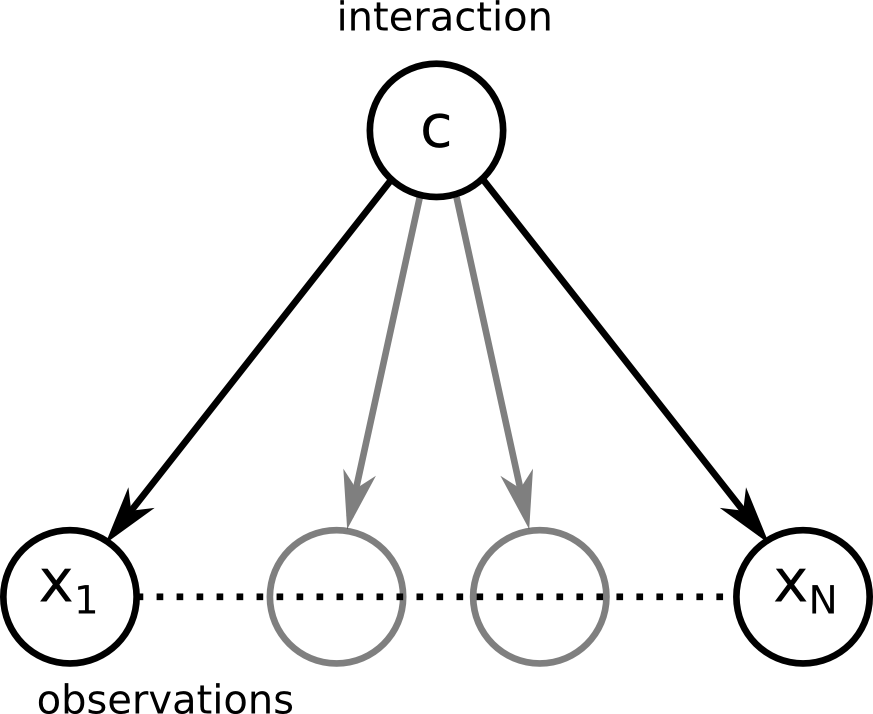
\includegraphics[width=0.6\textwidth]{naive.png}
    \caption{A belief network illustrating the Naive Bayes model, equivalent to that used for inference when weighting the interactions of the \ac{PPI} network.}
    \label{fig:naive}
\end{figure}

%updating on evidence? equations

%the importance of conservative estimates
The class label, interaction, is not observed in this model so we cannot solve to find the parameters.
%FIN: \ac{PPI} or not
To define the model, the only way to proceed is to manually define them by conservatively estimating the conditional true positive and false positive rates of the Bernoulli distributions.
Continuous distributions, such as the classifier predictions or prediction databases, must be estimated using \ac{KDE}. 
%FIN: explain \ac{KDE} acronym 

%kernel density estimation, justification from Weka
Using \ac{KDE} in conjunction with Naive Bayes is the approach used by Weka to deal with arbitrary conditional distributions\autocite{john_estimating_1995}.
%FIN: you need to explain what Weka is 
Unfortunately, this distribution is estimated using samples labeled using the protein interaction databases, so we cannot be fully confident in its predictions.
As before, a conservative estimate of its accuracy is applied through increasing the smoothing bandwidth.

\section{Measures applied to weighted and unweighted \ac{PPI} networks}

%why do we want to try weighted networks? and intro
It is hoped that a weighted graph will provide new insight into the interactions of proteins in the active zone.
%FIN: I think at this stage you need a refresher to the reader on what active zone you are talking about
For this reason, comparing the unweighted and weighted cases of the graph produced is a major goal of this project.
The following sections describe this process and the measures applied to both graphs.

\subsection{Community detection}
\label{communitydetection}
%FIN: section needs expansion in the areas you have noted 
%description of each of the algorithms available
%three:
%  Geodesic edge Betweenness
%  Random edge Betweenness
%  Spectral Betweenness
Three algorithms were identified for use in this project for community detection, the first two are described in \textcite{newman_finding_2004}.
Geodesic edge betweenness and random edge betweenness are based on betweenness measures to partition the graph, making them optimisation approaches.
The third, spectral modularity, was the chosen algorithm in this project.

%with reference to Colin's paper, why this is a good choice
The original advantages of spectral modularity techniques were better results in less time than competing methods in \textcite{newman_modularity_2006}.
In a recent paper, this method was compared favourably to other methods in terms of CPU time\autocite{mcleanunpub}.
Although it detected fewer communities, it maintained a higher modularity score.

%community detection code, what it does, which algorithm was used
%pending use - will see if I have time to use more than one

\subsection{Normalised Mutual Information}

%NMI theory, what is a measure of
Mutual information intuitively is the reduction in uncertainty about one random variable by observing another
Defined in terms of entropy it is\autocite{mackay_information_2003}:

%could move that citation next to the equation?
\begin{align}
    I(X;Y) = H(X) - H(X|Y)
\end{align}

Where $H(X)$ is the entropy of the random variable $X$ and $H(X|Y)$ is the conditional entropy of $X$ given $Y$.

In the case of the function we are using to perform this from Scikit-learn the mutual information is normalised by $\sqrt{H(X)\times H(Y)}$\autocite{pedregosa_scikit-learn:_2011}.
This produces a value between zero and one which reflects the redundancy of the distributions - 1.0 being exactly the same and 0.0 being independent.

\subsection{Disease Enrichment}
\label{diseaseenrichment}

%Primer on what this test actually does
By linking the proteins in a cluster to known disease annotations it is possible to estimate the likelihood that a given community is involved in a particular disease.
The code being used produces a p-value to indicate this likelihood.
%FIN: explain a p-val? 

In the case of this project, due to the aims of the SYNSYS project and for simplicity, only two diseases were investigated: Schizophrenia and Alzheimer's.

%interaction between significance level and p-value


\section*{Conclusion}

This project involved a large number of varied techniques and algorithms being used on large data sets.
Many problems had to be solved in order to piece together the full project.
As each of these steps were sequential, the results section describes the results as they were gathered, in the same structure as seen above.
